% Preamble
\documentclass[11pt]{article}
\usepackage{perf}

% Document
\begin{document}

    \perfset{
    robust fast \\
    5    30 \\
    2     1 \\
    2     1 \\
    5    50 \\
    5     1 \\
    2     1 \\
    2     1 \\
    4     1 \\
    2     1 \\
    3     1 \\
    4    45 \\
    }

    \printperftable

    \vspace{1cm}
    \begin{tikzpicture}
        \begin{axis}[title=Performances,height=6cm]
            \addperformances
            \legend{robust, fast}
        \end{axis}
    \end{tikzpicture}

    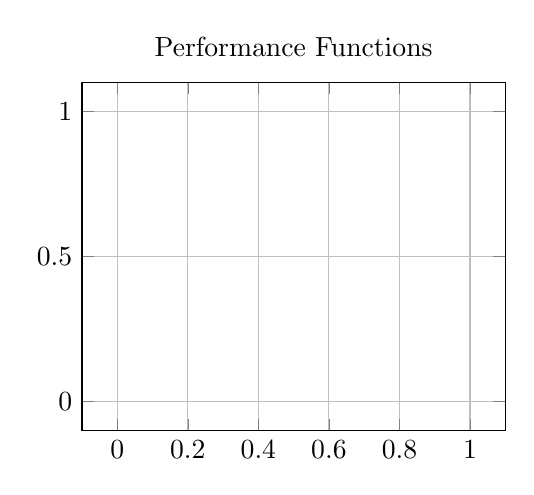
\begin{tikzpicture}
        \begin{axis}[title=Performance Functions,height=6cm,
        legend pos=outer north east,grid=both,no marks]
            \addprofiles{2}{10}
            \legend{robust,fast}
        \end{axis}
    \end{tikzpicture}


    %
    % Second set of data and plots
    %

    \perfset{
    better worse worst \\
    1    30  99\\
    1     2  10\\
    1     3  10\\
    1    50  999\\
    1     3  9 \\
    1     1  16383 \\
    16383 1 9999\\
    16383 2 9999 \\
    }

    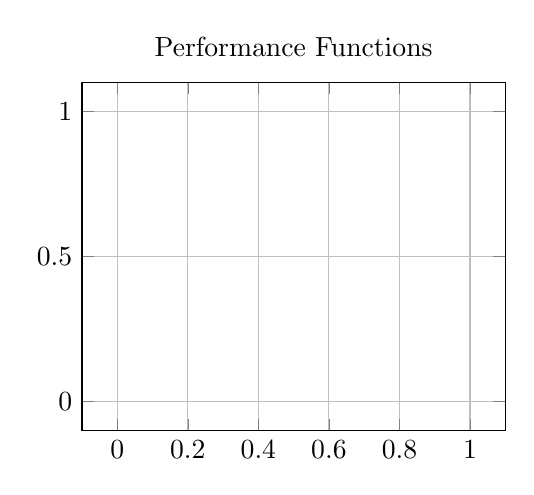
\begin{tikzpicture}
        \begin{axis}[title=Performance Functions,height=6cm,
        legend pos=outer north east,grid=both,no marks]
            \addprofiles{3}{15}
            \legend{better,worse,worst}
        \end{axis}
    \end{tikzpicture}


\end{document}